%Chapter 3
\chapter{Developing a simulation methodology}
\thispagestyle{empty}
\vspace{38em}
\hrulefill
\\
\enquote*{\textit{Quote.}} - Somebody\\
\newpage
\section{Introduction}
\section{System investigation method}
	\subsection{Preamble}
		Developing a detailed simulation model of a compressed air network requires thorough comprehension of the inner workings of the system. This section will discuss the investigations required to obtain this understanding.
	\subsection{Data acquisition and verification} % 
		-Layouts, data from SCADA Instrumentation, etc.
	\subsection{Solutions to unavailable data}
	Parameters that are required to develop the simulation model, such as flows, pressures, specifications etc., may not be actively recorded by mine personnel or computer systems. In order to obtain this data it is necessary to investigate alternative sources.
	\par 
	Flow and pressure instrumentation measurements are most often not available throughout the air network. At points where these measurement are absent, estimations can be made from assumptions f
	\par 
	Air network specifications such as piping sizes and compressor parameters is often outdated or not recorded. Audits and manual investigations should be implemented to obtain this data. If these investigations are not possible estimations should be made using the available data.
	\par 
	
		- When instrumentation isn't available\\
		- locate leaks etc.\\
		- Estimate/ measure typical flows to sections\\
		- Audits\\
		- Manual measurements required
	\subsection{Mining schedule}
		- Identify typical mining procedures and philosophies that influence the consumption of compressed air.\\
		- eg. Drilling throughout the day or shift, different types of shift, air requirements
	\subsection{Summary}
\section{Model development and verification}
	\subsection{Preamble}
	This section will discuss the development of a compressed air simulation model in \gls{stb}.
	\subsection{Compressed air component models}
		\gls{stb} 
		\subsubsection{Pipes}
		\subsubsection{Ambient conditions}
		Ambient air condition will vary greatly throughout a mining air network. Pressure and temperature increases with depth  as a result of auto compression. Underground conditions maintain relatively stable compared to the surface. Air condition can effect the performance of the network therefore it is important to include them in the model.
		\par 
		Surface conditions can be obtained through average weather measurements taken near or at the required site or estimated from measurements at other location. Underground conditions can be obtained through measurements if available. Alternative the conditions can be estimated by using the depth below the surface. The obtained pressure, temperature and humidity parameters can be imported directly into the air boundary component.
		\paragraph{Compressor model}\leavevmode\\
		In \gls{stb} three compressor models are available with varying complexity: air compressor, dynamic compressor and positive displacement compressor. When used, the compressor component is added to the air network in the arrangement shown in figure \ref{fig: Compressor models}. The Compressor is connected to the inlet air source via an inlet pipe and air node and to the rest of the network via an air node and outlet pipe. This is is to allow the inlet and outlet parameters and conditions to be be monitored and controlled.
		\begin{figure}[h]
			\centering
			\fbox{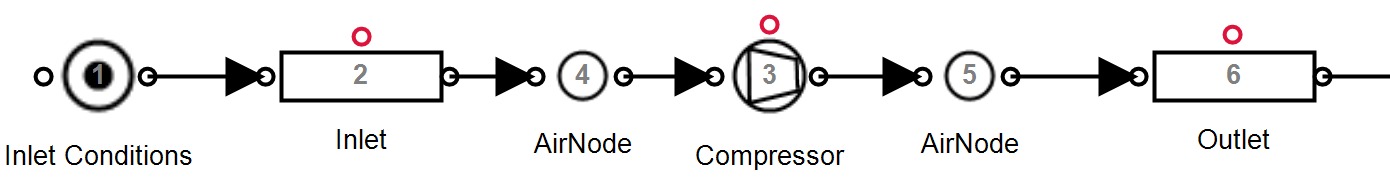
\includegraphics[trim =-4cm 0 -4cm 0cm, width=\textwidth]{Images/3/Compressors}}
			\caption{Modelling a compressor in \gls{stb}.}
			\label{fig: Compressor models}
		\end{figure}
		\par
		 The air compressor model is a general, simplified compressor model. This model requires minimal user inputs by making several assumptions. This is useful when parameters for a compressor are not available. Or when doing a quick preliminary simulation. However it is not ideal for detailed simulations which require more precision.
		 \par 
		 The dynamic and positive displacement compressor models are more complex, taking into account factors such as heat caused by polytopic compression and inefficiencies. The models do still make several assumptions for example, the compressor efficiency at different loads is assumed to remain the same. This can cause the operation of the model can differ slightly from the real life compressor.
		 \par
		 For most scenarios, the dynamic compressor model will be suitable. This models fits a quadratic curve through three points to obtain an equation for corrected mass flow as a function of the pressure ratio. This characteristic compressor curve as shown in figure \ref{fig: Compressor Curve} can be accurately estimated even when only one data point is available by making approximations for the zero flow and pressure points on the curve.\footnote{TEMM International, \enquote*{Process toolbox - Thermal hydraulic simulation flow solver,} User Manual, 2014} 
			\begin{figure}[h]
				\centering
				\fbox{% GNUPLOT: LaTeX picture with Postscript
\begingroup
  \makeatletter
  \providecommand\color[2][]{%
    \GenericError{(gnuplot) \space\space\space\@spaces}{%
      Package color not loaded in conjunction with
      terminal option `colourtext'%
    }{See the gnuplot documentation for explanation.%
    }{Either use 'blacktext' in gnuplot or load the package
      color.sty in LaTeX.}%
    \renewcommand\color[2][]{}%
  }%
  \providecommand\includegraphics[2][]{%
    \GenericError{(gnuplot) \space\space\space\@spaces}{%
      Package graphicx or graphics not loaded%
    }{See the gnuplot documentation for explanation.%
    }{The gnuplot epslatex terminal needs graphicx.sty or graphics.sty.}%
    \renewcommand\includegraphics[2][]{}%
  }%
  \providecommand\rotatebox[2]{#2}%
  \@ifundefined{ifGPcolor}{%
    \newif\ifGPcolor
    \GPcolortrue
  }{}%
  \@ifundefined{ifGPblacktext}{%
    \newif\ifGPblacktext
    \GPblacktextfalse
  }{}%
  % define a \g@addto@macro without @ in the name:
  \let\gplgaddtomacro\g@addto@macro
  % define empty templates for all commands taking text:
  \gdef\gplbacktext{}%
  \gdef\gplfronttext{}%
  \makeatother
  \ifGPblacktext
    % no textcolor at all
    \def\colorrgb#1{}%
    \def\colorgray#1{}%
  \else
    % gray or color?
    \ifGPcolor
      \def\colorrgb#1{\color[rgb]{#1}}%
      \def\colorgray#1{\color[gray]{#1}}%
      \expandafter\def\csname LTw\endcsname{\color{white}}%
      \expandafter\def\csname LTb\endcsname{\color{black}}%
      \expandafter\def\csname LTa\endcsname{\color{black}}%
      \expandafter\def\csname LT0\endcsname{\color[rgb]{1,0,0}}%
      \expandafter\def\csname LT1\endcsname{\color[rgb]{0,1,0}}%
      \expandafter\def\csname LT2\endcsname{\color[rgb]{0,0,1}}%
      \expandafter\def\csname LT3\endcsname{\color[rgb]{1,0,1}}%
      \expandafter\def\csname LT4\endcsname{\color[rgb]{0,1,1}}%
      \expandafter\def\csname LT5\endcsname{\color[rgb]{1,1,0}}%
      \expandafter\def\csname LT6\endcsname{\color[rgb]{0,0,0}}%
      \expandafter\def\csname LT7\endcsname{\color[rgb]{1,0.3,0}}%
      \expandafter\def\csname LT8\endcsname{\color[rgb]{0.5,0.5,0.5}}%
    \else
      % gray
      \def\colorrgb#1{\color{black}}%
      \def\colorgray#1{\color[gray]{#1}}%
      \expandafter\def\csname LTw\endcsname{\color{white}}%
      \expandafter\def\csname LTb\endcsname{\color{black}}%
      \expandafter\def\csname LTa\endcsname{\color{black}}%
      \expandafter\def\csname LT0\endcsname{\color{black}}%
      \expandafter\def\csname LT1\endcsname{\color{black}}%
      \expandafter\def\csname LT2\endcsname{\color{black}}%
      \expandafter\def\csname LT3\endcsname{\color{black}}%
      \expandafter\def\csname LT4\endcsname{\color{black}}%
      \expandafter\def\csname LT5\endcsname{\color{black}}%
      \expandafter\def\csname LT6\endcsname{\color{black}}%
      \expandafter\def\csname LT7\endcsname{\color{black}}%
      \expandafter\def\csname LT8\endcsname{\color{black}}%
    \fi
  \fi
    \setlength{\unitlength}{0.0500bp}%
    \ifx\gptboxheight\undefined%
      \newlength{\gptboxheight}%
      \newlength{\gptboxwidth}%
      \newsavebox{\gptboxtext}%
    \fi%
    \setlength{\fboxrule}{0.5pt}%
    \setlength{\fboxsep}{1pt}%
\begin{picture}(9360.00,4032.00)%
    \gplgaddtomacro\gplbacktext{%
      \colorrgb{0.00,0.00,0.00}%
      \put(814,704){\makebox(0,0)[r]{\strut{}$0$}}%
      \colorrgb{0.00,0.00,0.00}%
      \put(814,1261){\makebox(0,0)[r]{\strut{}$100$}}%
      \colorrgb{0.00,0.00,0.00}%
      \put(814,1818){\makebox(0,0)[r]{\strut{}$200$}}%
      \colorrgb{0.00,0.00,0.00}%
      \put(814,2375){\makebox(0,0)[r]{\strut{}$300$}}%
      \colorrgb{0.00,0.00,0.00}%
      \put(814,2932){\makebox(0,0)[r]{\strut{}$400$}}%
      \colorrgb{0.00,0.00,0.00}%
      \put(814,3489){\makebox(0,0)[r]{\strut{}$500$}}%
      \colorrgb{0.00,0.00,0.00}%
      \put(946,484){\makebox(0,0){\strut{}$0$}}%
      \colorrgb{0.00,0.00,0.00}%
      \put(1948,484){\makebox(0,0){\strut{}$2$}}%
      \colorrgb{0.00,0.00,0.00}%
      \put(2950,484){\makebox(0,0){\strut{}$4$}}%
      \colorrgb{0.00,0.00,0.00}%
      \put(3952,484){\makebox(0,0){\strut{}$6$}}%
      \colorrgb{0.00,0.00,0.00}%
      \put(4954,484){\makebox(0,0){\strut{}$8$}}%
      \colorrgb{0.00,0.00,0.00}%
      \put(5956,484){\makebox(0,0){\strut{}$10$}}%
      \colorrgb{0.00,0.00,0.00}%
      \put(6958,484){\makebox(0,0){\strut{}$12$}}%
      \colorrgb{0.00,0.00,0.00}%
      \put(7960,484){\makebox(0,0){\strut{}$14$}}%
      \colorrgb{0.00,0.00,0.00}%
      \put(8962,484){\makebox(0,0){\strut{}$16$}}%
      \csname LTb\endcsname%
      \put(5455,3043){\makebox(0,0)[l]{\strut{}$f(x) = -2.586x^2 + 7.788x + 494$}}%
    }%
    \gplgaddtomacro\gplfronttext{%
      \csname LTb\endcsname%
      \put(176,2235){\rotatebox{-270}{\makebox(0,0){\strut{}Mass flow ($kg^3/s/\sqrt(k)/Bar$)}}}%
      \put(4954,154){\makebox(0,0){\strut{}Pressure ratio}}%
    }%
    \gplbacktext
    \put(0,0){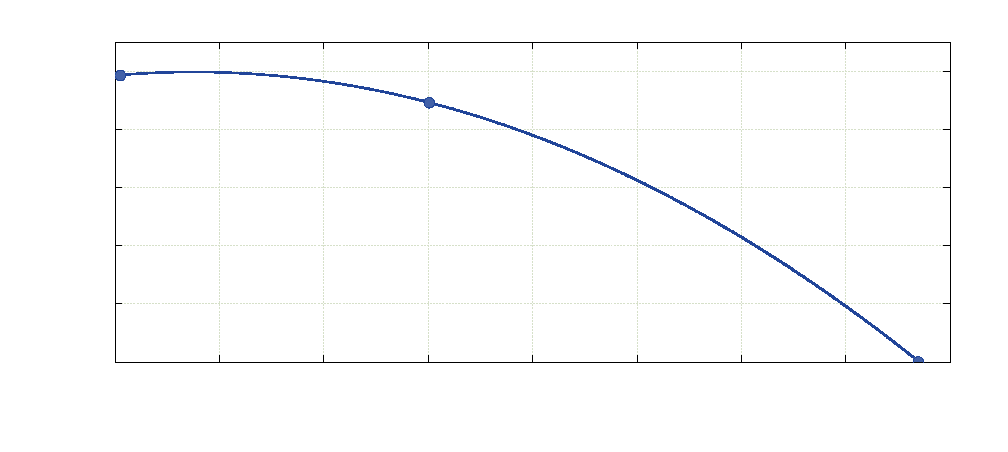
\includegraphics{Graphs/3/AproxCurve/AproxCurve}}%
    \gplfronttext
  \end{picture}%
\endgroup
}
				\caption{Estimating the characteristic curve of a compressor using the dynamic compressor model.}
				\label{fig: Compressor Curve}
			\end{figure}
		\subsubsection{Demand/leak}
	
		\subsubsection{Controllers}
		Compressed air networks rely on controllers
\begin{figure}[h]
	\centering
	\fbox{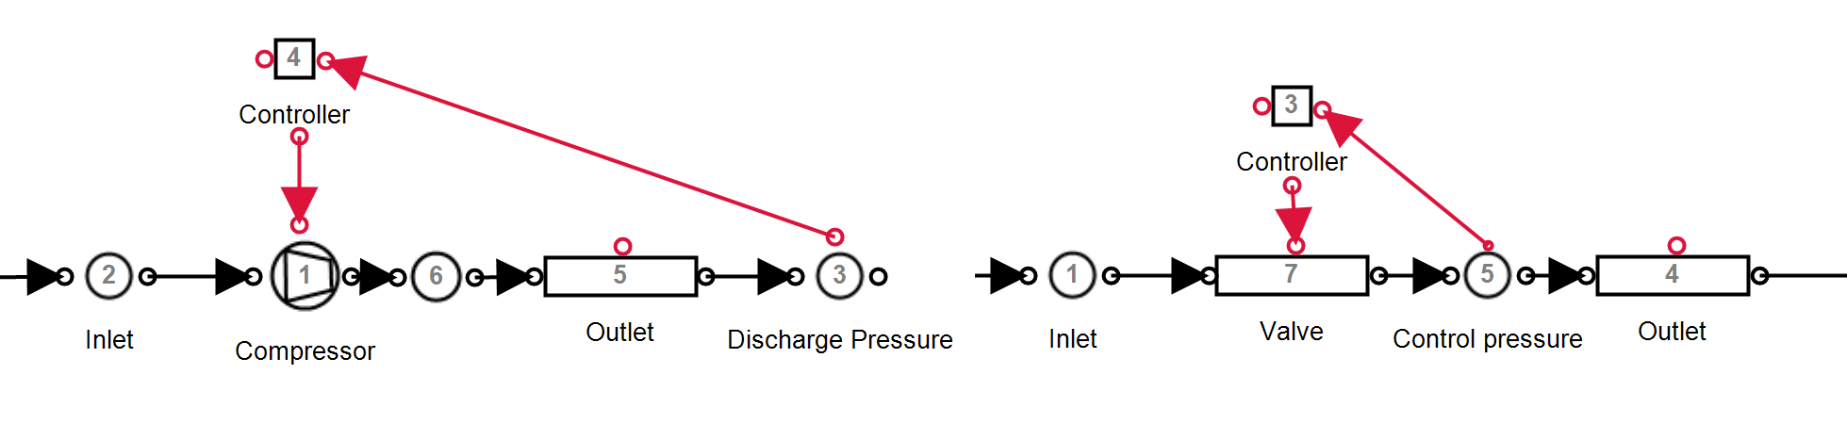
\includegraphics[trim =-4cm 0 -4cm 0cm, width=\textwidth]{Images/3/Controller}}
	\caption{Control components in \gls{stb}.}
	\label{fig: Controller models}
\end{figure}
		\subsubsection{After Cooling}
	\subsection{Simulation inputs}
		-Discuss inputs of the simulation, (compressor setpoints, ambient conditions, demands)
	\subsection{Verification of simulation model}
		- Steps to validate  the model accuracy .\\
		- Compare parameters to actuals
	\subsection{Summary}
\section{Approach to method implementation}
	\subsection{Preamble}
		- This section will discuss the approach to implementation and analysis of the simulation.
	\subsection{Analyses of data}
		- Baseline vs Optimised comparison \\
	\subsection{Quantifying operational improvements}
		- Estimating cost savings
	\subsection{Summary}
\section{Conclusion}
